
\section{Resoconto attivita\textsubscript{G} di verifica}
In questa sezione possaimo vedere gli esiti delle attività di verifica durante la fase di Avvio e Analisi dei Requisiti, e quello che per ora stiamo facendo nella fase di Progettazione Architetturale.\\
Il nostro cruscotto è presente al seguente indirizzo:\\ \url{https://sites.google.com/view/three-way-milkshake-dashboard}.\\PS: utilizzare un account non universitario per poterlo visualizzare correttamente.
\subsection{Avvio}
\subsubsection{Verifica dei Processi}
\begin{figure}[H]
	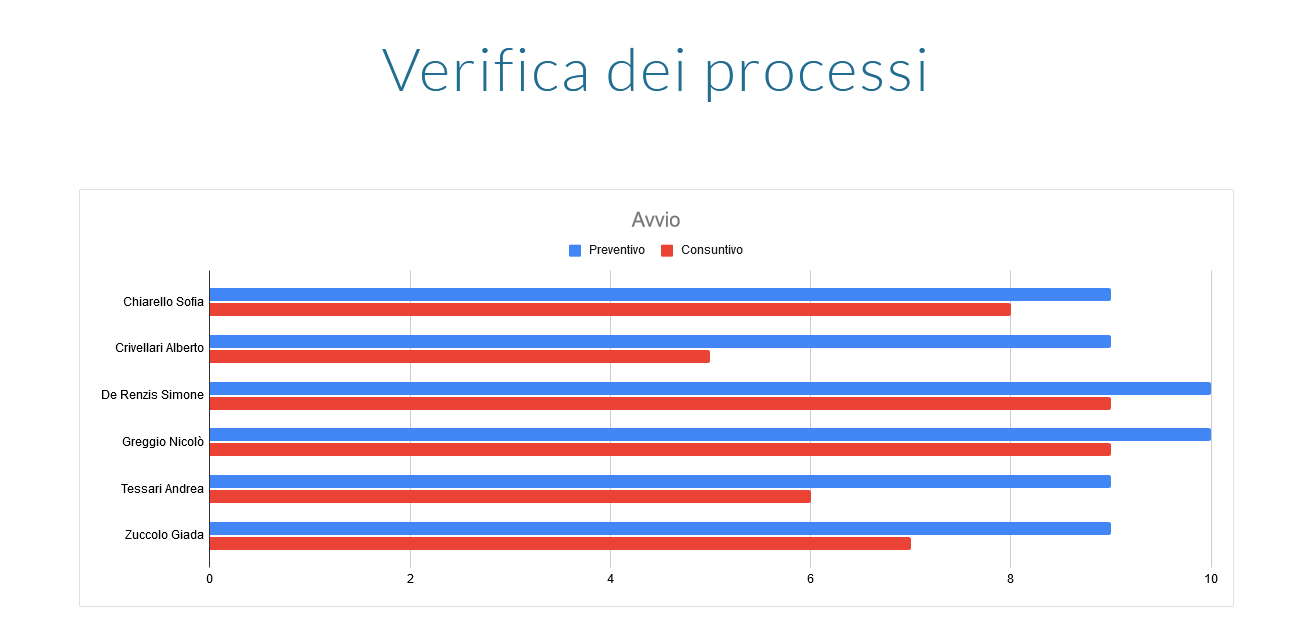
\includegraphics[scale=0.5]{res/images/cruscotto/avvio_1.png}
\end{figure}
\begin{figure}[H]
	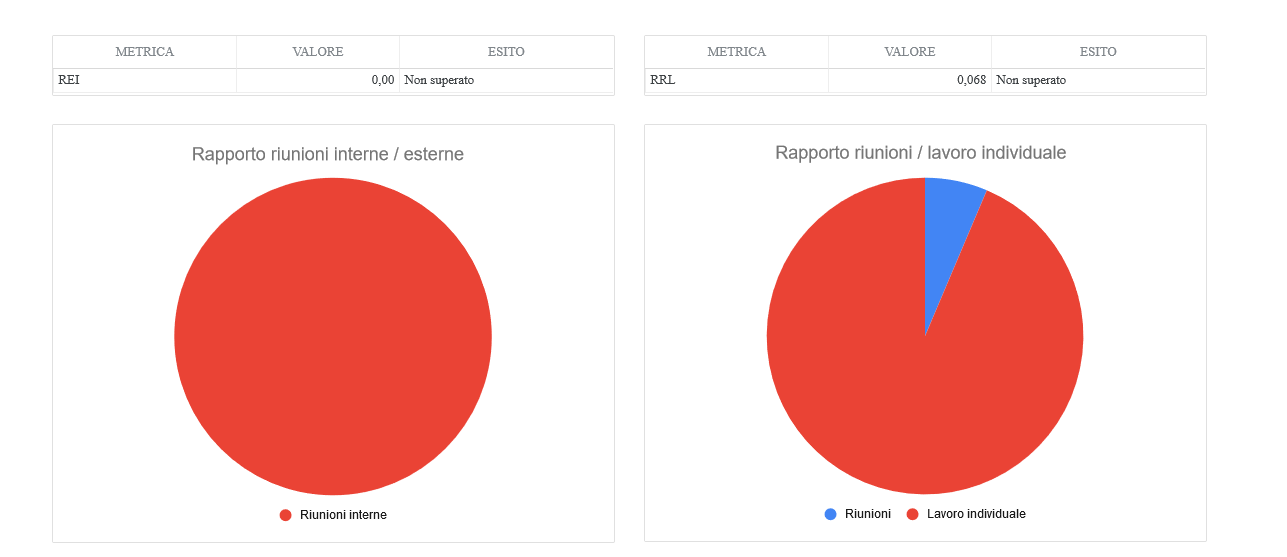
\includegraphics[scale=0.5]{res/images/cruscotto/avvio_2.png}
\end{figure}
\begin{figure}[H]
	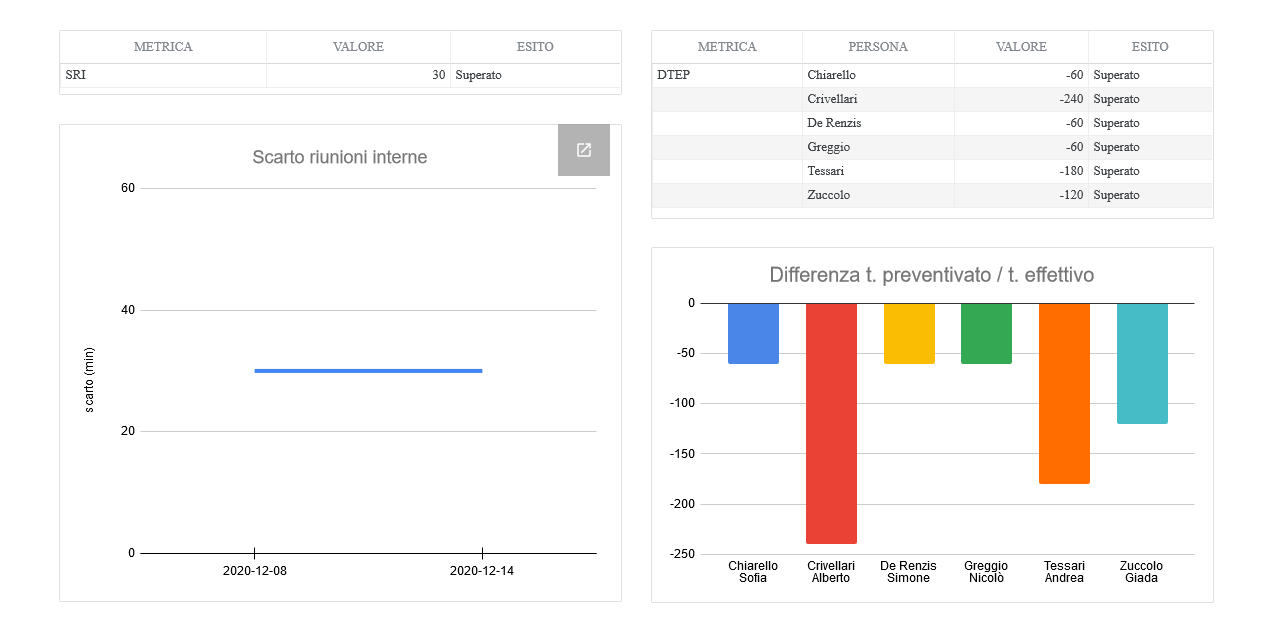
\includegraphics[scale=0.5]{res/images/cruscotto/avvio_3.png}
\end{figure}
\begin{figure}[H]
	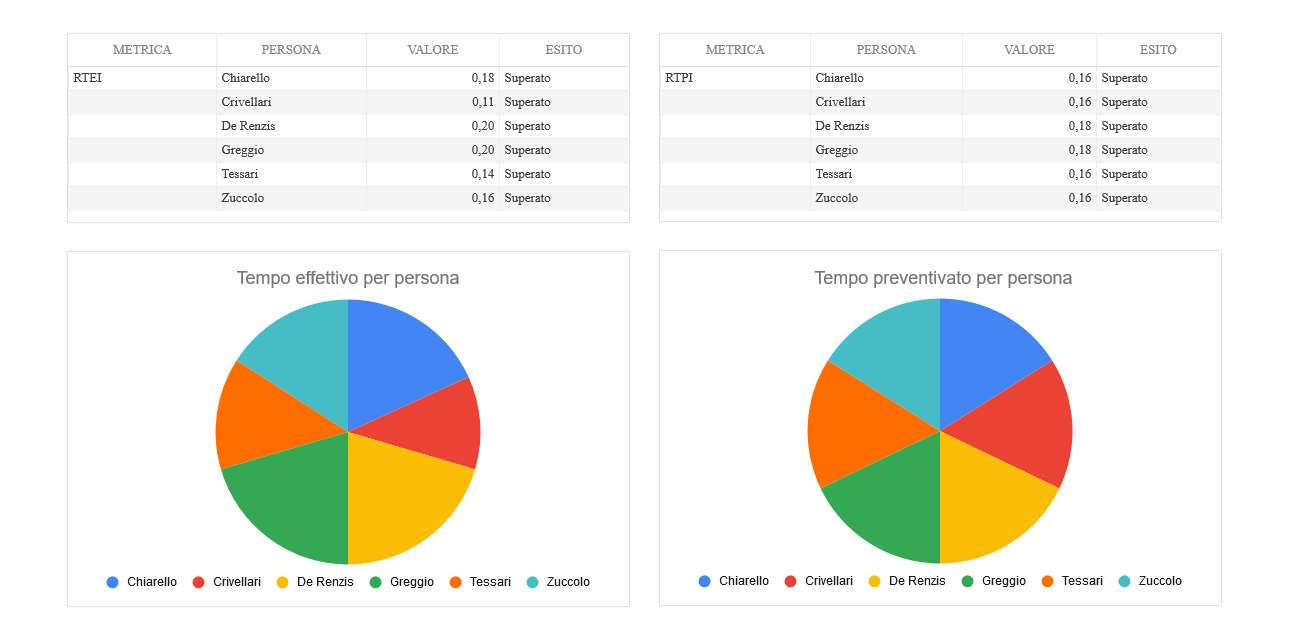
\includegraphics[scale=0.5]{res/images/cruscotto/avvio_4.png}
\end{figure}
\subsubsection{Verifica della Documentazione}
\begin{figure}[H]
	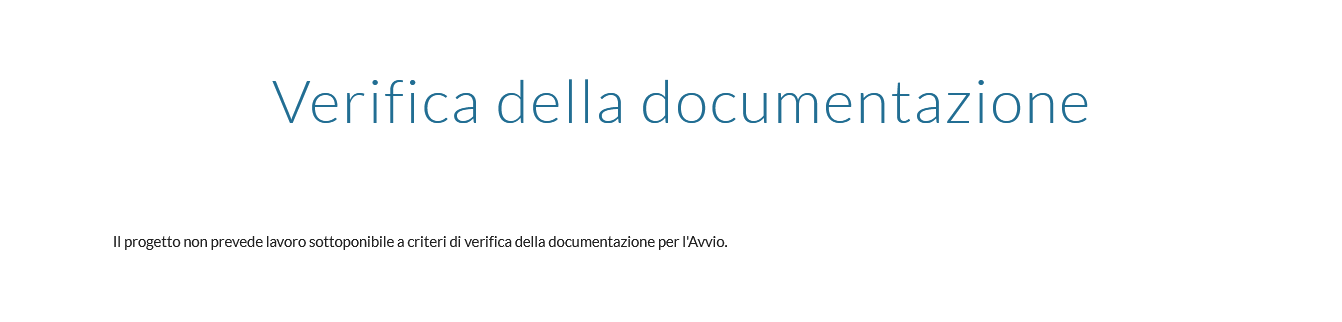
\includegraphics[scale=0.55]{res/images/cruscotto/avvio_5.png}
\end{figure}
\subsubsection{Verifica del Prodotto}
\begin{figure}[H]
	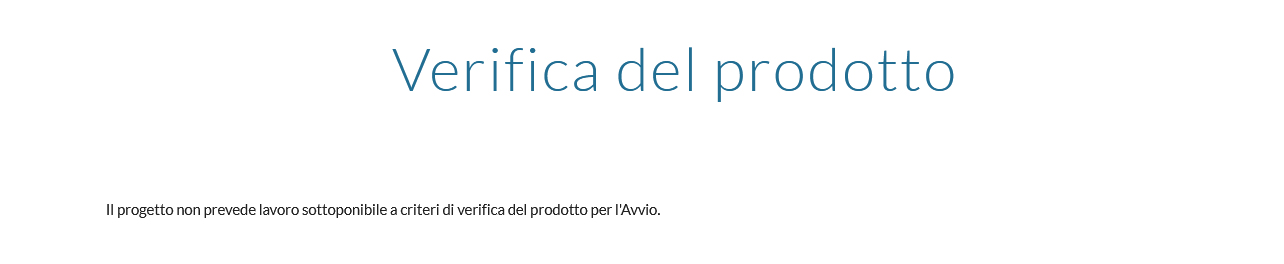
\includegraphics[scale=0.55]{res/images/cruscotto/avvio_6.png}
\end{figure}
\pagebreak
\subsection{Analisi Dei Requisiti}
\subsubsection{Verifica dei Processi}
\begin{figure}[H]
	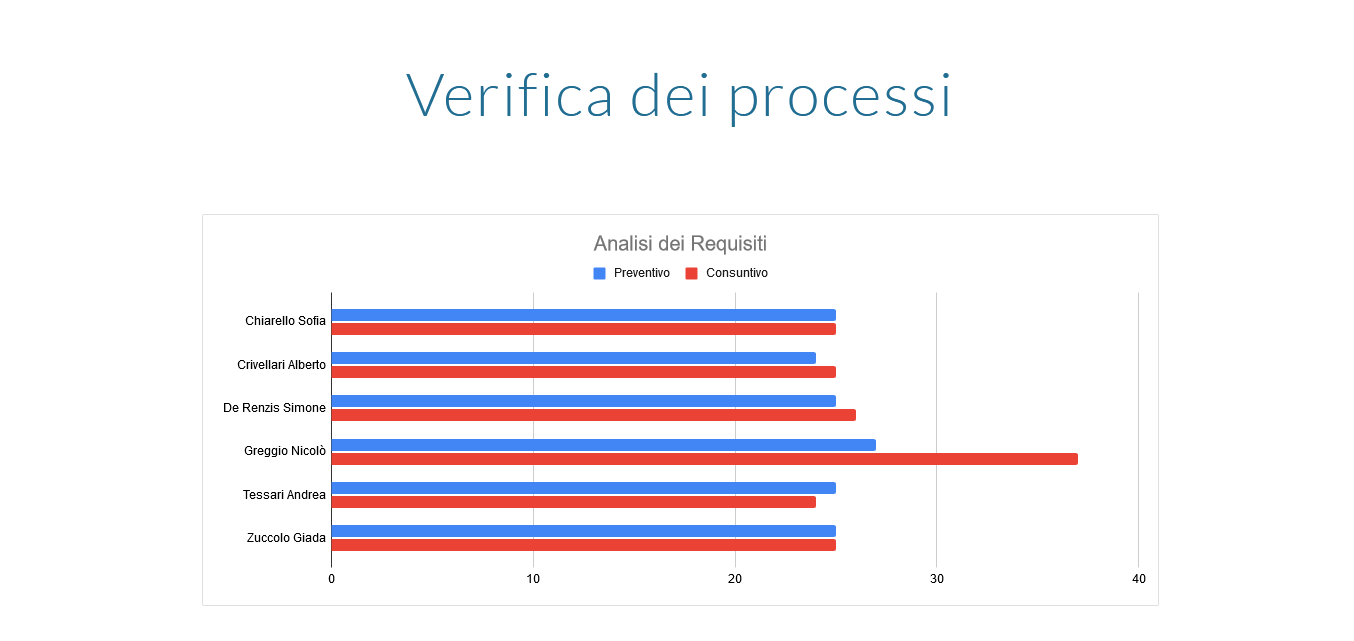
\includegraphics[scale=0.5]{res/images/cruscotto/adr_1.png}
\end{figure}
\begin{figure}[H]
	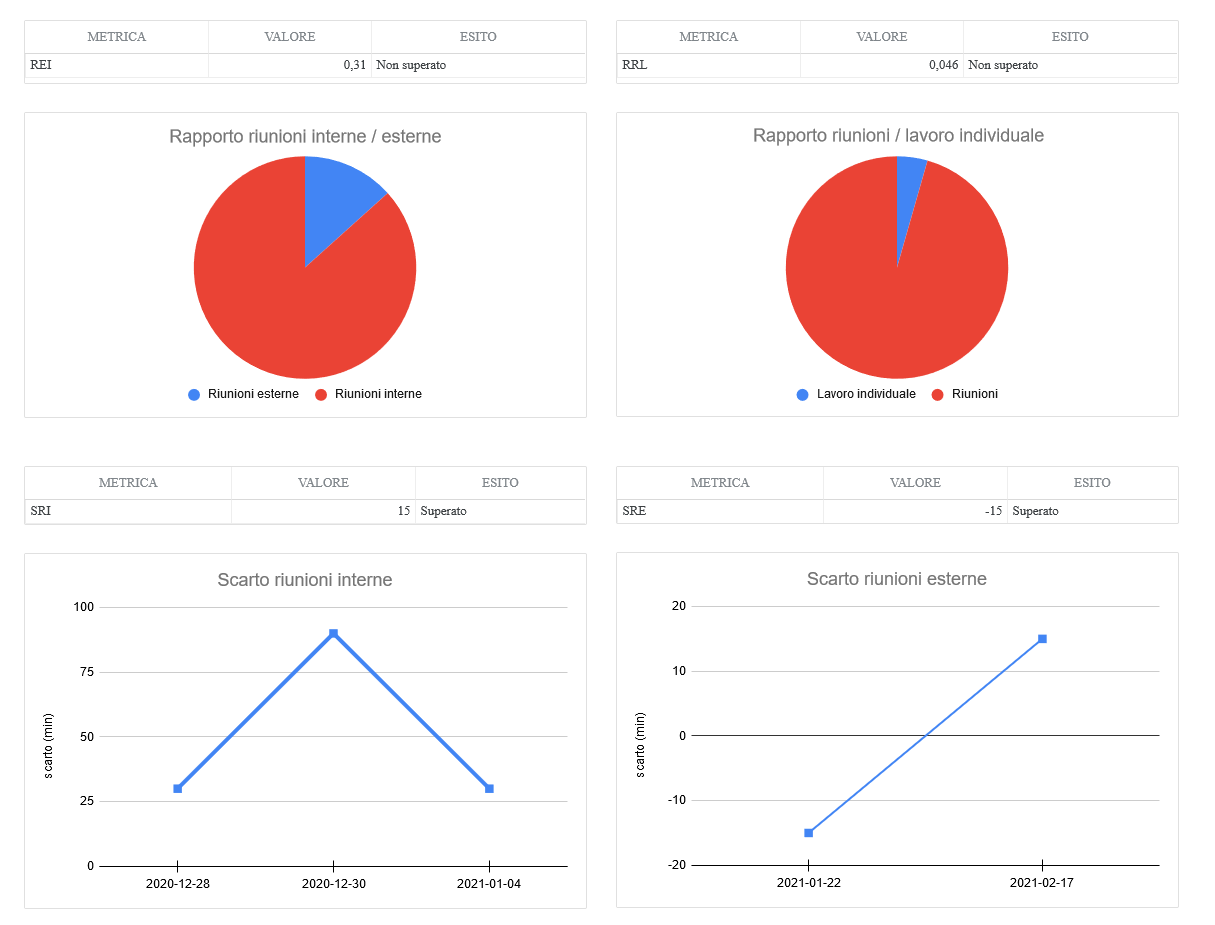
\includegraphics[scale=0.4]{res/images/cruscotto/adr_2.png}
\end{figure}
\begin{figure}[H]
	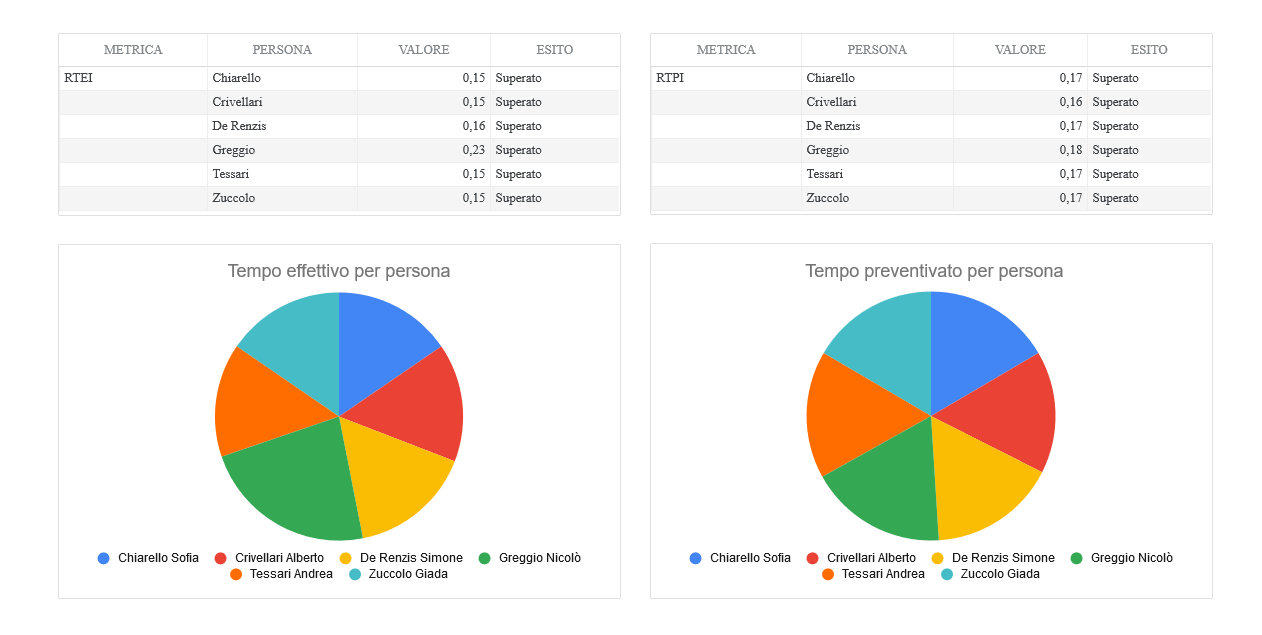
\includegraphics[scale=0.5]{res/images/cruscotto/adr_3.png}
\end{figure}
\begin{figure}[H]
	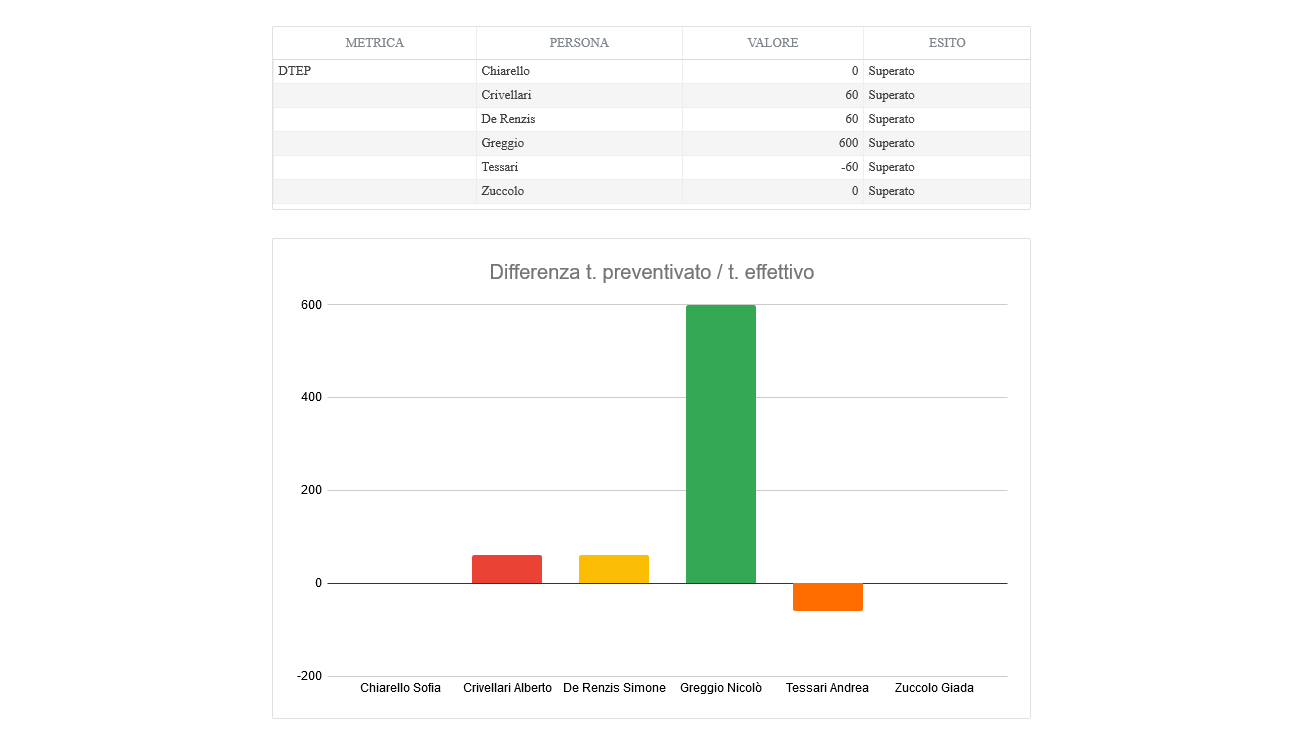
\includegraphics[scale=0.5]{res/images/cruscotto/adr_4.png}
\end{figure}
\subsubsection{Verifica della Documentazione}
\begin{figure}[H]
	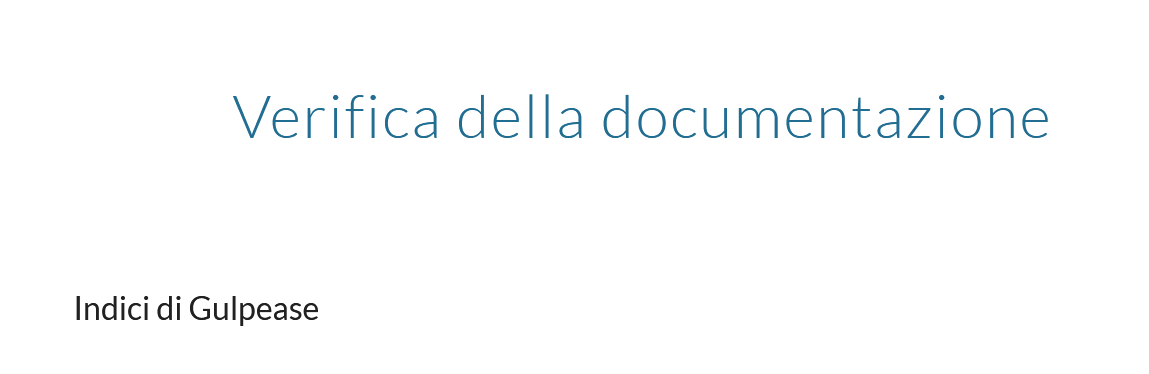
\includegraphics[scale=0.5]{res/images/cruscotto/adr_5.png}
\end{figure}
\begin{figure}[H]
	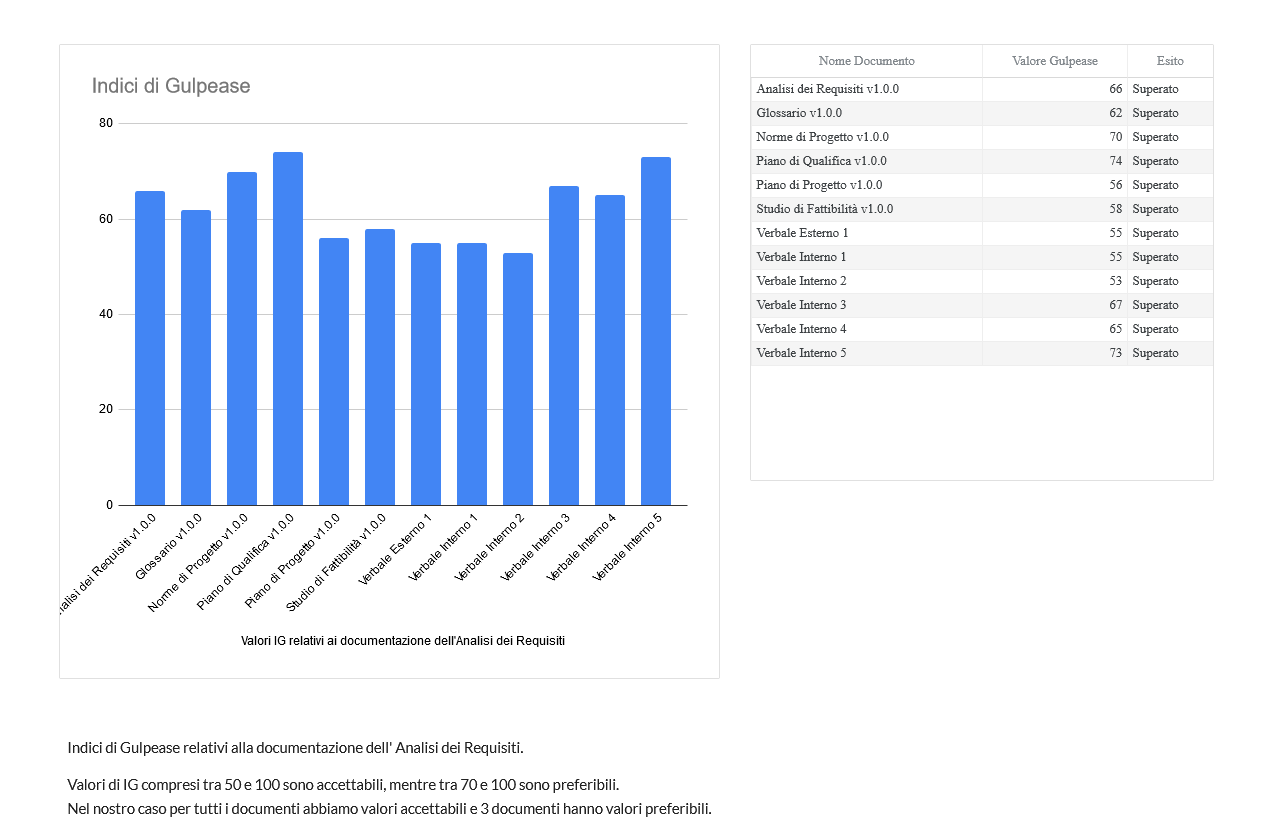
\includegraphics[scale=0.5]{res/images/cruscotto/adr_6.png}
\end{figure}
\subsubsection{Verifica del Prodotto}
\begin{figure}[H]
	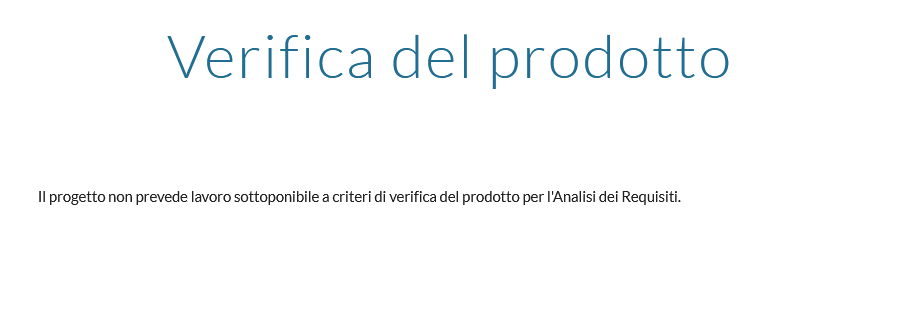
\includegraphics[scale=0.55]{res/images/cruscotto/adr_7.png}
\end{figure}
\pagebreak
\subsection{Progettazione Architetturale}
\subsubsection{Verifica dei Processi}
\begin{figure}[h]
	\centering
	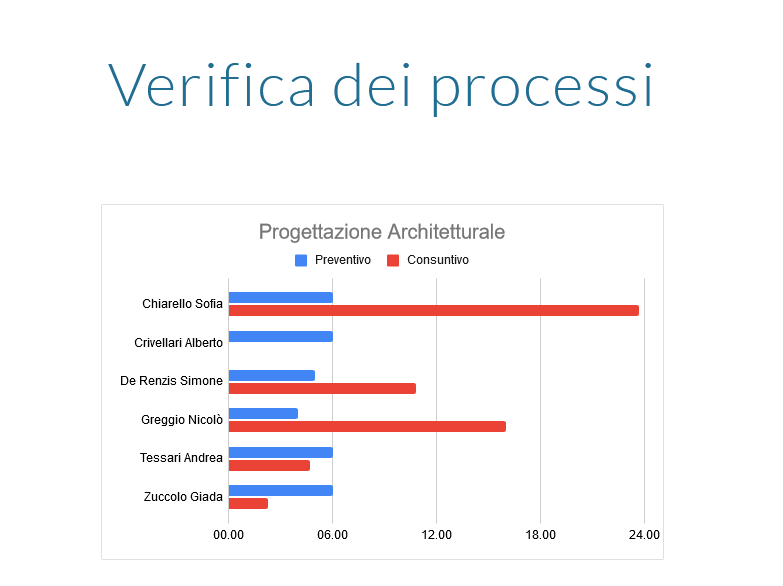
\includegraphics[scale=0.6]{res/images/cruscotto/pa_1.png}
\end{figure}
\begin{figure}[H]
	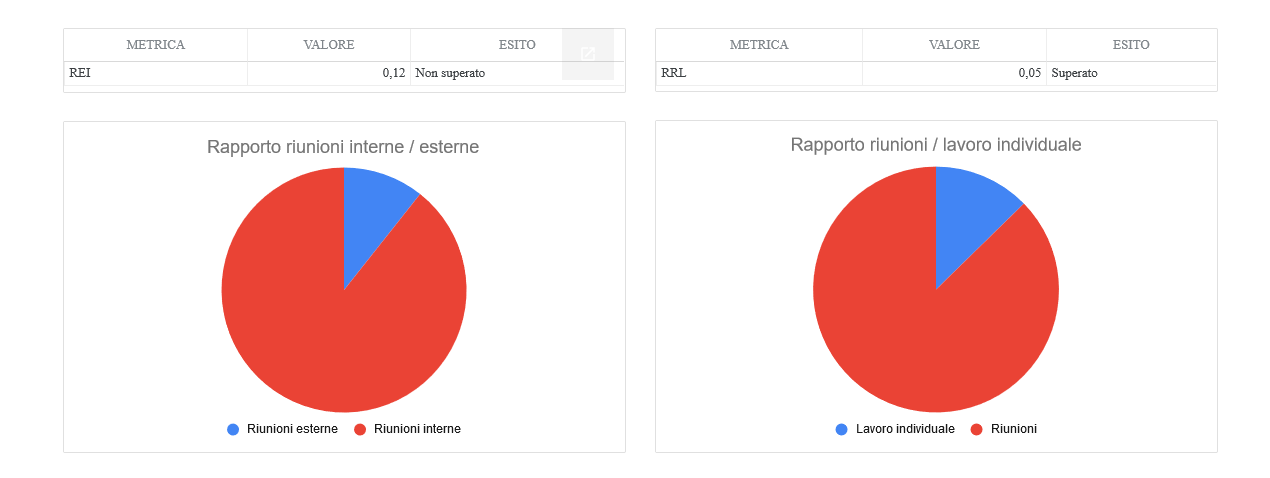
\includegraphics[scale=0.5]{res/images/cruscotto/pa_2.png}
\end{figure}
\begin{figure}[H]
	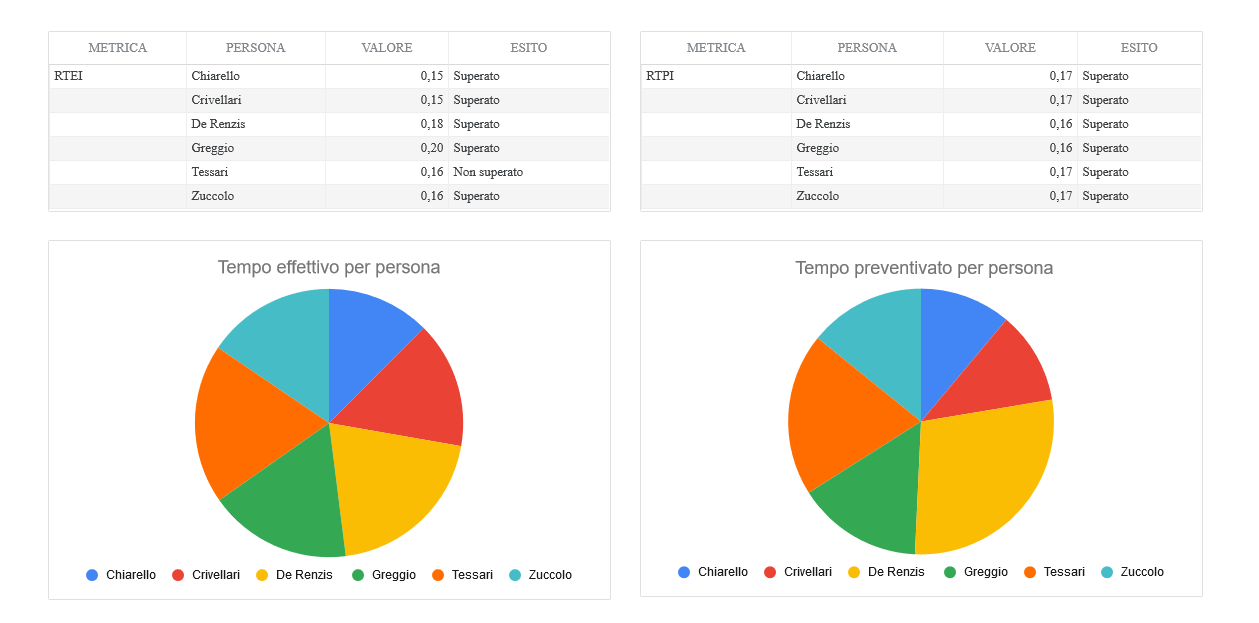
\includegraphics[scale=0.5]{res/images/cruscotto/pa_3.png}
\end{figure}
\begin{figure}[H]
	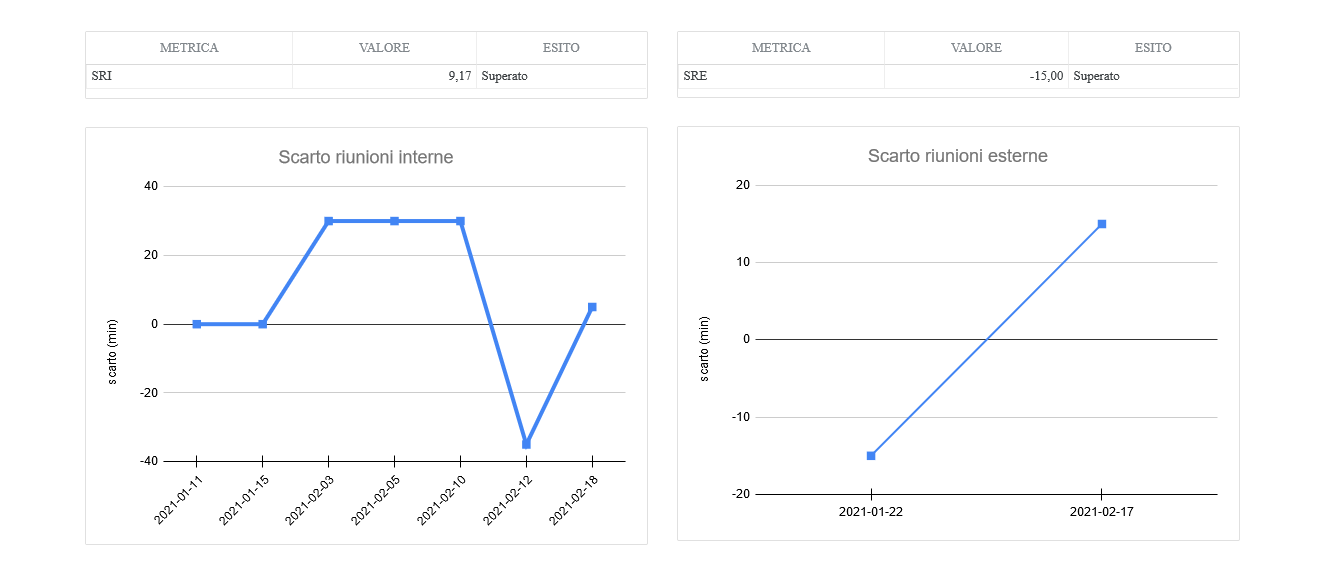
\includegraphics[scale=0.5]{res/images/cruscotto/pa_4.png}
\end{figure}
\begin{figure}[H]
	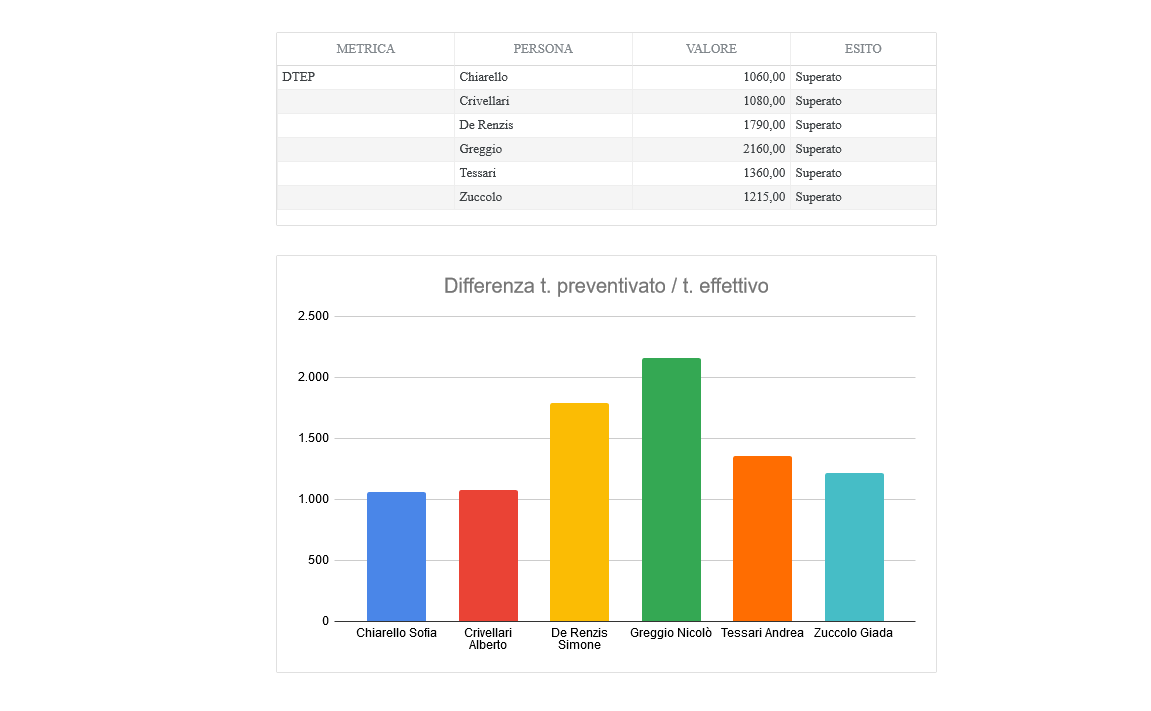
\includegraphics[scale=0.5]{res/images/cruscotto/pa_5.png}
\end{figure}
\begin{figure}[H]
	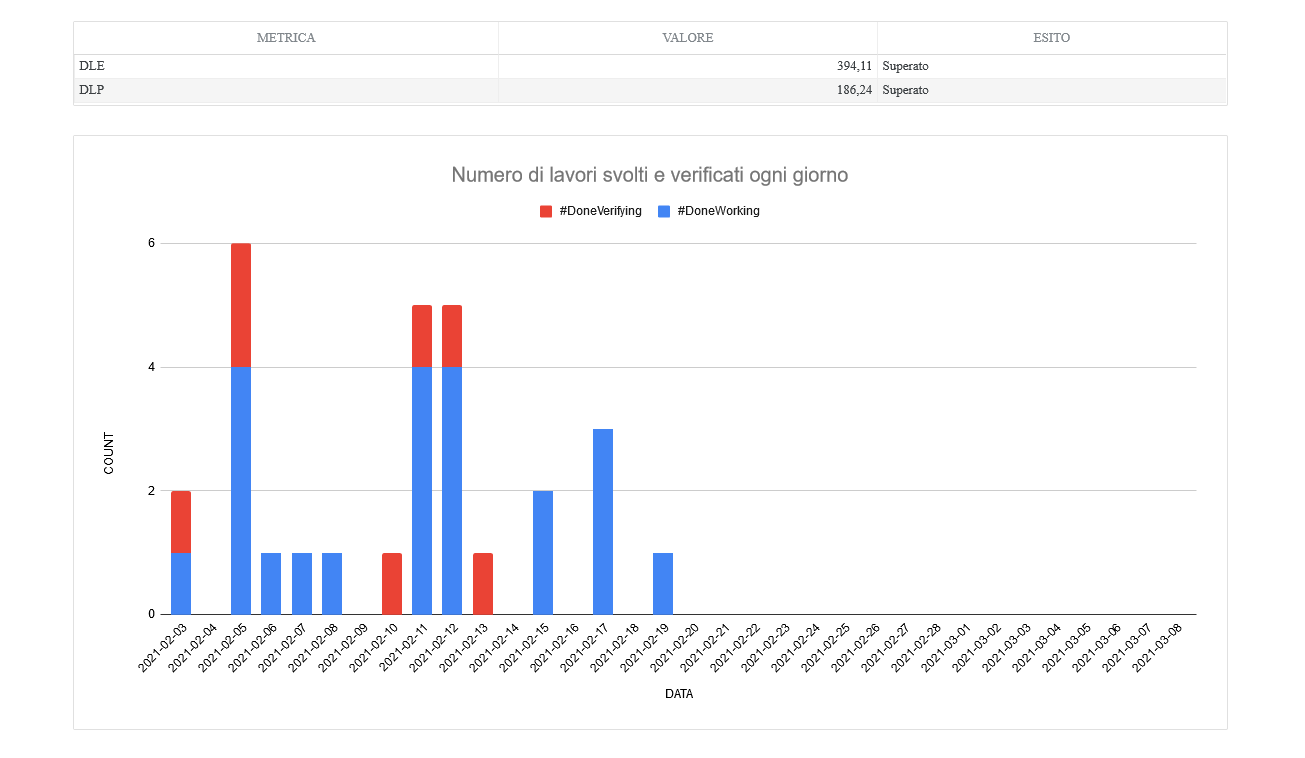
\includegraphics[scale=0.5]{res/images/cruscotto/pa_6.png}
\end{figure}
\begin{figure}[H]
	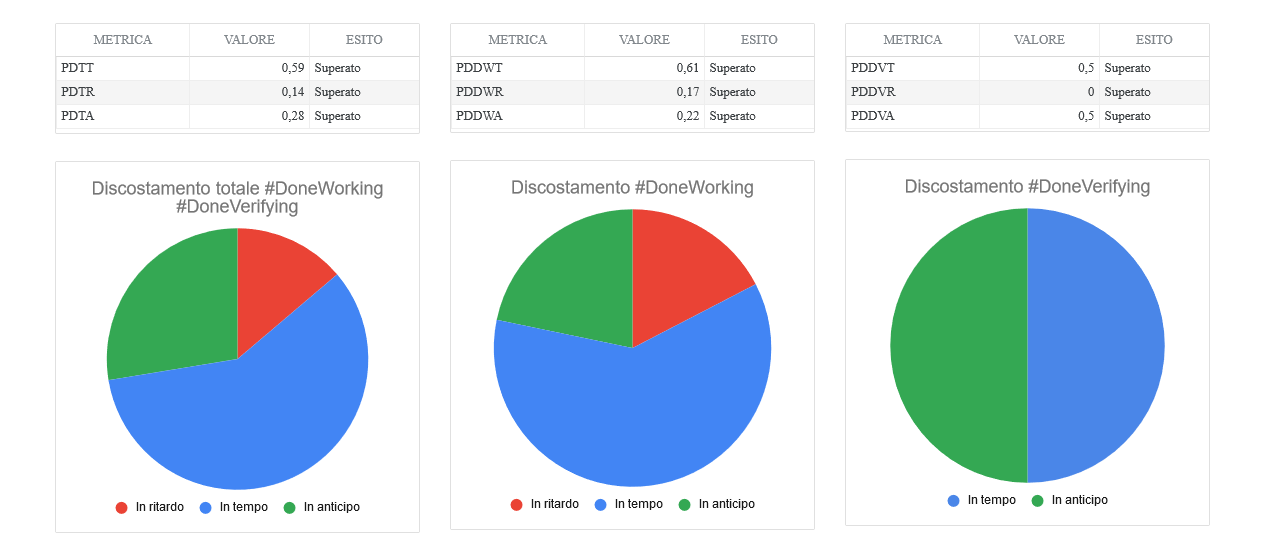
\includegraphics[scale=0.5]{res/images/cruscotto/pa_7.png}
\end{figure}
\pagebreak
\subsubsection{Verifica della Documentazione}
\begin{figure}[H]
	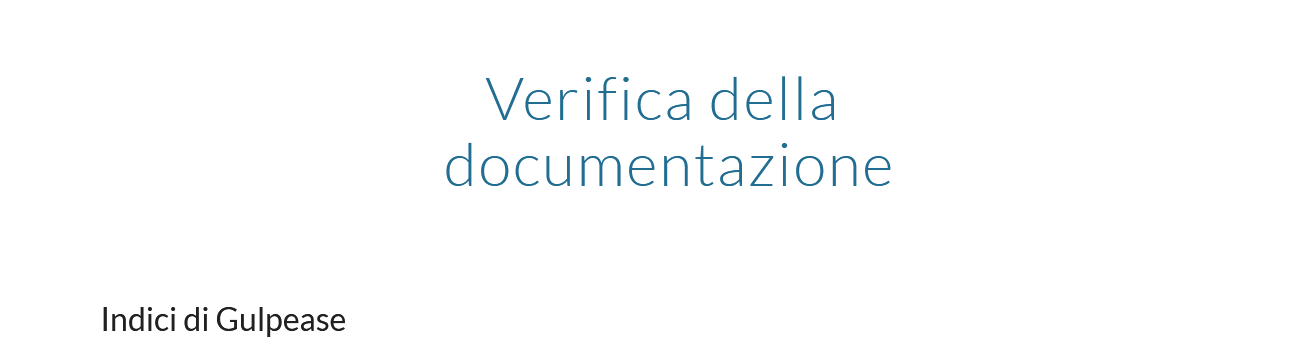
\includegraphics[scale=0.5]{res/images/cruscotto/pa_8.png}
\end{figure}
\begin{figure}[H]
	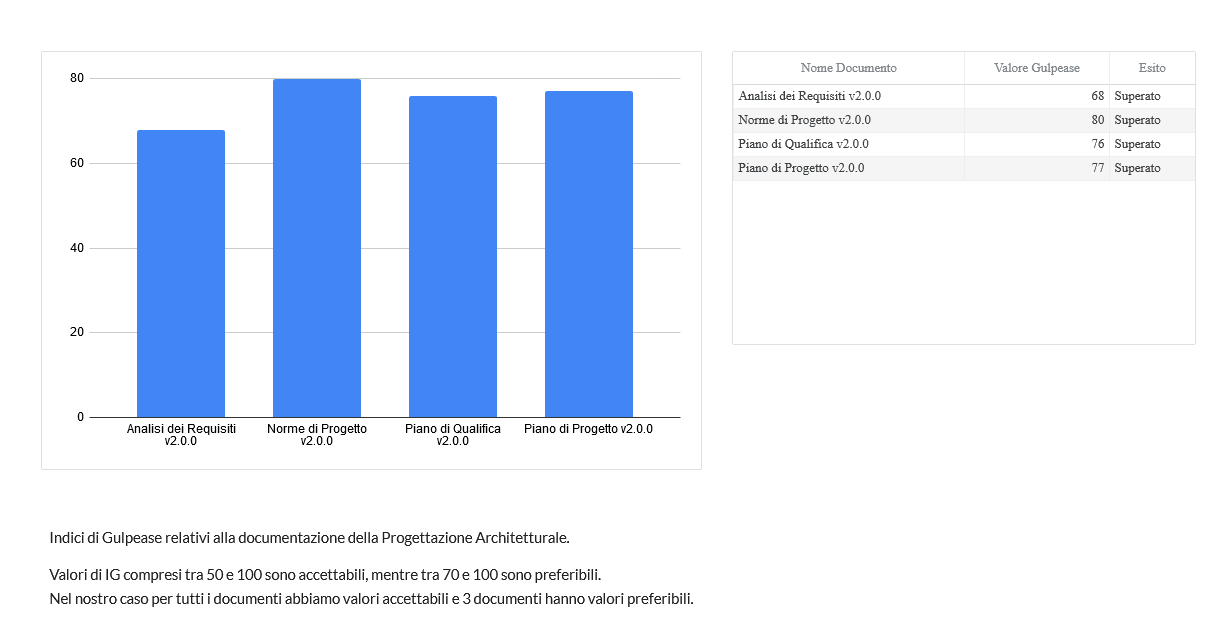
\includegraphics[scale=0.5]{res/images/cruscotto/pa_9.png}
\end{figure}
\subsubsection{Verifica del Prodotto}
\begin{figure}[H]
	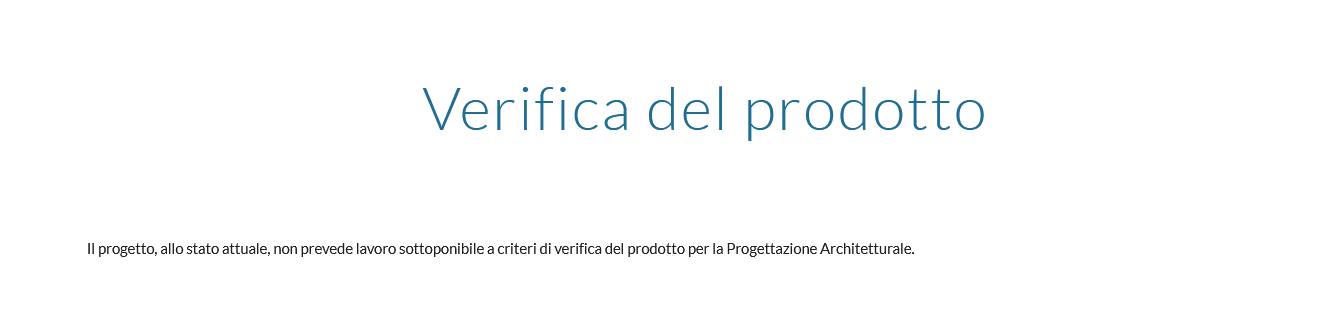
\includegraphics[scale=0.5]{res/images/cruscotto/pa_10.png}
\end{figure}
\pagebreak
\subsection{Osservazioni}
Osservando gli esiti delle attività di verifica delle varie fasi, possiamo migliorare la quantità di riunioni esterne col proponente e diminuire la quantità di riunioni interne.